\documentclass{beamer}  
\usepackage{amsmath}
\usepackage{graphicx}
\usepackage{url}
\usepackage{listings}
\usepackage{fancyvrb}
\usepackage[T1]{fontenc}
\usepackage{hyperref}
\mode<presentation>
{ \usetheme{Warsaw} }
\title{Maths
}

\author{League of Programmers}
\institute{ACA, IIT Kanpur}
\date{October 22, 2012}
 
\AtBeginSection[]  % "Beamer, do the following at the start of every section"
{
\begin{frame}<beamer> 
\frametitle{Outline} % make a frame titled "Outline"
\tableofcontents[currentsection]  % show TOC and highlight current section
\end{frame}
}

\begin{document}
%----------- titlepage ----------------------------------------------%
\begin{frame}
  \titlepage
\end{frame}

\section{Maths}

\begin{frame}[<+->]{GCD}
\begin{itemize}
  \item gcd(a, b): greatest integer divides both a and b
  \item If b|a then gcd(a,b) = b
  \item Otherwise a = bt+r for some t and r\\
  \begin{itemize}
    \item gcd(a,b) = gcd(b,r)
    \item gcd(a,b) = gcd(b,a\%b)
  \end{itemize}
  \item lcm(a,b) = (a*b)/gcd(a,b)
  \item Running time: O (log (a + b))
\end{itemize}
\end{frame}

\begin{frame}{GCD}
  \begin{block}{Recursive Implementation:}
  \tt{
    int gcd(int a, int b) \{\\
      \hspace{2mm} if (b==0)\\
	\hspace{5mm} return a;\\
      \hspace{2mm} else\\
	\hspace{5mm} return gcd(b,a\%b);\\
     \}
    }
  \end{block}
\end{frame}

\begin{frame}{GCD}
  \begin{block}{Iterative Implementation:}
  \tt{
    int gcd(int a, int b) \{\\
      \hspace{2mm} while(b) \{\\
	\hspace{5mm} int r = a \% b;\\
	\hspace{5mm} a = b;\\
	\hspace{5mm} b = r;\\
      \hspace{2mm} \}\\
      \hspace{2mm} return a;\\
     \}
    }
  \end{block}
\end{frame}

\begin{frame}[<+->]{Modular Exponentiation}
\begin{itemize}
  \item Compute $a^n$ in O(log n) time
  \item $a^n$ = 1, if n=0\\
	      \hspace{5mm} = a if n=1\\
	      \hspace{5mm} = $a^{{(n/2)}^2}$, if n =even\\
	      \hspace{5mm} = $a^{{((n-1)/2)}^2}$, if n = odd
\end{itemize}
\end{frame}

\begin{frame}{Modular Exponentiation}
  \begin{block}{Recursive Implementation:}
  \tt{
    double pow(double a, int n) \{\\
      \hspace{2mm} if(n == 0) return 1;\\
      \hspace{2mm} if(n == 1) return a;\\
      \hspace{2mm} double t = pow(a, n/2);\\
      \hspace{2mm} return t * t * pow(a, n\%2);\\
    \}
    }
  \end{block}
\end{frame}

\begin{frame}{Modular Exponentiation}
  \begin{block}{Iterative Implementation:}
  \alert{$a = a_0 + a_1*2 + a_2*2^2+...+a_k*2^k$}\\
  \tt{
    int result=1,power=a;\\
    while(!n) \{\\
      \hspace{2mm} if(n\&1)\\
	\hspace{5mm} result*=power;\\
      \hspace{2mm} power*=power;\\
      \hspace{2mm} n>>=1;\\
    \}
    }
  \end{block}
\end{frame}

\begin{frame}[<+->]{Fibonacci}
  \begin{block}{}
    \begin{itemize}
      \item $F_n = F_{n-1} + F_{n-2}$
      \item $\bigl(\begin{smallmatrix} F_n\\ F_{n-1} \end{smallmatrix} = [\begin{smallmatrix} 1&1\\ 1&0 \end{smallmatrix}] * \begin{smallmatrix} F_{n-1}\\ F_{n-2} \end{smallmatrix}\bigr)$
      \item $\bigl(\begin{smallmatrix} F_n\\ F_{n-1} \end{smallmatrix} = {[\begin{smallmatrix} 1&1\\ 1&0 \end{smallmatrix}]}^n * \begin{smallmatrix} F_{1}\\ F_{0} \end{smallmatrix}\bigr)$
      \item Compute the product in O(lg n) time
      \item \alert{Can be extended to support any linear recurrence with constant coefficients}
    \end{itemize}
  \end{block}
\end{frame}

\begin{frame}[<+->]{Binomial Coefficients}
  \begin{block}{}
    \begin{itemize}
      \item ${n \choose k}$ = Number of ways to choose k objects out of n distinguishable objects
      \item Computing ${n \choose k}$
	\begin{enumerate}
	  \item Compute using the following formula\\
	    \begin{center}${n \choose k}$ = $\frac{n(n-1) \dots (n-k+1)}{k!}$\end{center}
	  \item Use Pascal's triangle
	\end{enumerate}
      \item Cases:
	\begin{enumerate}
	  \item Both n and k are small\\
	    Use either solution
	  \item n is big, but k or n-k is small\\
	    Use Solution 1 (carefully)
	\end{enumerate}
    \end{itemize}
  \end{block}
\end{frame}

\begin{frame}[<+->]{Lucas Theorem}
  \begin{block}{}
    \begin{itemize}
      \item The Lucas' theorem expresses the remainder of division of the binomial coefficient ${m \choose n}$ by a prime number p in terms of the base p expansions of the integers m and n.
      \item For non-negative integers m and n and a prime p, the following congruence relation holds:\\
	\begin{center}${m \choose n} = \prod_{i=0}^k {m_i \choose n_i}  (mod p)$\end{center}
	where\\
	$m = m_{k}p^{k} + m_{k-1}p^{k-1} + \dots + m_1p + m_0 $\\
	and\\
	$n = n_{k}p^{k} + n_{k-1}p^{k-1} + \dots + n_1p + n_0 $\\
	are base p expansions of m and n respectively.
    \end{itemize}
  \end{block}
\end{frame}

\begin{frame}[<+->]{Problem}
  \begin{block}{Problem 1}
    Find the number of strings of length "N" made up of only 3 characters - a, b, c such that "a" occurs at least "min\_a" times and at most "max\_a" times, "b" occurs at least "min\_b" times and at most "max\_b" times and "c" occurs at least "min\_c" times and at most "max\_c" times. Note that all permutations of same string count as 1, so "abc" is same as "bac".\\
    \url{http://www.spoj.pl/problems/DCEPC702/}
  \end{block}
\end{frame}

\begin{frame}[<+->]{Problem}
  \begin{block}{Problem 2}
    The main idea is to find a geometrical interpretation for the problem in which we should calculate the number of paths of a special type. More precisely, if we have two points A, B on a plane with integer coordinates, then we will operate only with the shortest paths between A and B that pass only through the lines of the integer grid and that can be done only in horizontal or vertical movements with length equal to 1.
    \begin{figure}
	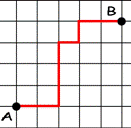
\includegraphics[scale=0.30]{figure41.png}
	\caption{1}
      \end{figure}
  \end{block}
\end{frame}

\begin{frame}[<+->]{Problem}
  \begin{block}{Solution}
    Solution: All paths between A and B have the same length equal to n+m (where n is the difference between x-coordinates and m is the difference between y-coordinates). We can easily calculate the number of all the paths between A and B:\\
    \hspace{2mm} Ans: ${m+n \choose n}$ or ${m+n \choose m}$
  \end{block}
\end{frame}

\begin{frame}[<+->]{Problem}
  \begin{block}{Problem 3}
    Let's solve a famous problem using this method. The goal is to find the number of Dyck words with a length of 2n. What is a Dyck word? It's a string consisting only of n X's and n Y's, and matching this criteria: each prefix of this string has more X's than Y's. For example, "XXYY" and "XYXY" are Dyck words, but "XYYX" and "YYXX" are not.\\
    \begin{center}{\bf OR}\end{center}
    Find the number of ways to arrange n '(' and n ')' brackets such that at each index, the number of '(' is never less than the number of ')'
  \end{block}
\end{frame}

\begin{frame}[<+->]{Problem}
  \begin{block}{Solution}
    Solution: Total ways: ${2n \choose n}$\\
    \hspace{10mm} Incorrect ways: ${2n \choose n-1}$\\
    Ans: Catalan number $\frac{1}{n+1}{2n \choose n}$
  \end{block}
\end{frame}

\begin{frame}[<+->]{Modular Arithmetic}
  \begin{block}{}
    \begin{itemize}
      \item (x+y) mod n = ((x mod n) + (y mod n))mod n
      \item (x-y) mod n = ((x mod n) - (y mod n))mod n
      \item (x*y) mod n = (x mod n)*(y mod n)mod n
      \item \alert{But, (x/y) mod n = ((x mod n)/(y mod n))mod n, not always true}
      \item $x^y$ mod n = ${(x mod n)}^y$ mod n
    \end{itemize}
  \end{block}
\end{frame}

\begin{frame}[<+->]{Multiplicative Inverse}
  \begin{block}{}
    \begin{itemize}
      \item $x^{-1}$ is the inverse of x modulo n if $x*x^{-1} \equiv 1(modn)$
      \item $5^{-1} \equiv 3(mod7)$ because $5*3 \equiv 15 \equiv 1(mod7)$
      \item May not exist (e.g. Inverse of 2 mod 4)
      \item \alert{Exists iff gcd(x,n) = 1}
      \item gcd(a,b)=ax+by for some integers x, y
      \item If gcd(a,n)=1, then ax + ny = 1 for some x, y
      \item Taking modulo n gives $ax \equiv 1(modn)$
      \item Given a,b, Finding x and y, such that ax+by = d is done by {\bf Extended Euclid's algorithm}
    \end{itemize}
  \end{block}
\end{frame}

\begin{frame}[<+->]{Prime Seive}
  \begin{block}{}
    \begin{itemize}
      \item Idea: every composite number n has a prime factor $p \leq \sqrt{n}$. So let us assume that all numbers are prime. But if we come across a prime factor of a number, we immediately know that it is not a prime. If there is no prime factor of a number n in the range [2 \dots n-1] then it must be prime.
    \end{itemize}
  \end{block}
\end{frame}

\begin{frame}[<+->]{Prime Seive}
  \begin{block}{Implementation}
      {\bf Generate all primes in range [1..n]}\\
      \tt{
	  For i=1 to n\\
	    \hspace{2mm} prime[i]=1\\
	  Prime[1]=0\\
	  For i=2 to $\sqrt{n}$\\
	    \hspace{2mm} if(prime[i])\\
	      \hspace{5mm} for j = i to n/i\\
		\hspace{8mm} prime[i*j]=0
	}\\
      At the end of this step, all numbers i which are prime have prime[i]=1. Others have prime[i]=0.
\end{block}
\end{frame}

\begin{frame}[<+->]{Prime Number Theorem}
  \begin{block}{}
  \begin{itemize}
      \item Prime number Theorem\\
      Number of primes till n $\sim$ n/logn
      \item Maximum number of prime factors of n = log n
  \end{itemize}
\end{block}
\end{frame}

\begin{frame}[<+->]{Euler Torient Function}
  \begin{block}{}
  \begin{itemize}
    \item $\phi(n)$ = Number of positive integers less than or equal to n which are coprime to n
    \item $\phi(ab) = \phi(a)*\phi(b)$
      \begin{itemize}
	\item For a prime p, $\phi(p) = p-1$
	\item For a prime p, $\phi(p^k) = p^k-p^{k-1} = p^k(1-\frac{1}{p})$
      \end{itemize}
    \item $N = (p_1^{k_1})*(p_2^{k_2})*...*(p_t^{k_t})$
      \begin{itemize}
	\item $\phi(n)=p_1^{a_1}p_2^{a_2}.. p_t^{a_t} ) = n*(1-\frac{1}{p_1})*(1-\frac{1}{p_2})* \dots *(1-\frac{1}{p_t})$\\
	$\equiv \phi(n)=p_1^{a_1}p_2^{a_2}.. p_t^{a_t} ) = n*\frac{(p_1-1)*(p_2-1)..(p_t-1)}{(p_1 p_2..p_t)}$
      \end{itemize}
  \end{itemize}
\end{block}
\end{frame}

\begin{frame}[<+->]{Euler Torient Function}
  \begin{block}{Seive for $\phi(n)$}
  \begin{itemize}
    \item Run prime sieve once and store result in primes[1..n]
    \item 
    \tt{
	for(i=1 to n) phi[i]=i\\
	for(i=2 to n)\\
	  \hspace{2mm} if(prime[i])\\
	    \hspace{5mm} for(j=1 to n/i)\\
	      \hspace{8mm} phi[i*j]=phi[i*j]*(i-1)/i
	}
    \item This algo runs in O(n log log n) time, but we will make improvements to show how you can at times optimize your code.
  \end{itemize}
\end{block}
\end{frame}

\begin{frame}[<+->]{Euler Torient Function}
  \begin{block}{Seive for $\phi(n)$}
  \begin{itemize}
    \item Question: Do we really need to generate list of all primes?
    \item Answer : No
    \item 
    \tt{
	for(i=1 to n) phi[i]=i\\
	for(i=2 to n)\\
	  \hspace{2mm} if(phi[i]==i)\\
	    \hspace{5mm} for(j=i to n;j+=i)\\
	      \hspace{8mm} phi[j] = (phi[j]/i)*(i-1);\\
	}
  \end{itemize}
\end{block}
\end{frame}

\begin{frame}[<+->]{Fermat's Little Theorem}
  \begin{block}{}
  \begin{itemize}
    \item If p is a prime number, then for any integer a that is coprime to n, we have $a^p \equiv a (mod p)$\\
    \item This theorem can also be stated as: If p is a prime number and a is coprime to p, then $a^{p-1} \equiv 1 (mod p)$
  \end{itemize}
\end{block}
\end{frame}

\begin{frame}[<+->]{Euler's Theorem}
  \begin{block}{}
  \begin{itemize}
    \item Euler's Theorem is a genaralization for Fermat's little theorem when a and n are co-prime
    \item If $x \equiv y (mod \phi(n))$, then $ax \equiv ay (mod n)$.
    \item $a^{\phi(n)} \equiv 1 (mod n)$ (actual theorem is a generalization of the above)
  \end{itemize}
\end{block}
\end{frame}

\begin{frame}[<+->]{Other results}
    If $n = p_1^{a_1}*p_2^{a_2}*...*p_t^{a_t}$, then\\
      \begin{itemize}
      \item The number of its positive divisors equals $(a_1 + 1) * (a_2 + 1) * ... * (a_t + 1)$
      \item Sum of the divisors of n equals\\
      $\sum_{d|n} = \prod_{i=1}^t {p_i^{m_i + 1} - 1 \over p_i - 1}$
      \end{itemize}
\end{frame}
\begin{frame}[<+->]{Miller-Rabin Test (Primality Testing)}
  \begin{block}{}
    Input: n > 1, an odd integer to test for primality.\\
    write n-1 as $2^s·d$ by factoring powers of 2 from n-1\\
    repeat for all : a $\in$ [2,n-2]\\
      \hspace{3mm} If $a^d \neq 1$ mod n and $a^{2^r}.d \neq -1$ mod n for all $r \in [0, s − 1]$\\
      \hspace{3mm} then return composite\\
    Return prime
\end{block}
\begin{block}{}
\begin{itemize}
  \item \small{if n < 9,080,191, it is enough to test a = 31 and 73;}
  \item \small{if n < 4,759,123,141, it is enough to test a = 2, 7, and 61;}
  \item \small{if n < 2,152,302,898,747, it is enough to test a = 2, 3, 5, 7, and 11;}
  \item \small{if n < 3,474,749,660,383, it is enough to test a = 2, 3, 5, 7, 11, and 13;}
  \item \small{if n < 341,550,071,728,321, it is enough to test a = 2, 3, 5, 7, 11, 13, and 17.}
\end{itemize}
\end{block}
\end{frame}

\section{Probability}
\begin{frame}[<+->]{Mathematical Expectation}
  \begin{block}{}
    \begin{itemize}
      \item For a discrete variable X with probability function P(X), the expected value E[X] is given by $\sum_i x_i*P(x_i)$ the summation runs over all the distinct values xi that the variable can take.
      \item The rule of "linearity of of the expectation" says that E[x1+x2] = E[x1] + E[x2].
      \item It is important to understand that "expected value" is not same as "most probable value" - rather, it need not even be one of the probable values.
    \end{itemize}
\end{block}
\end{frame}

\begin{frame}[<+->]{Mathematical Expectation}
  \begin{block}{Example}
    \begin{itemize}
      \item For a six-sided die, the expected number of throws to get each face at least once?
	  \item It's (6/6)+(6/5)+(6/4)+(6/3)+(6/2)+(6/1) = 14.7.
      \item Logic: The chance of rolling a number you haven't yet rolled when you start off is 1, as any number would work. Once you've rolled this number, your chance of rolling a number you haven't yet rolled is 5/6. Continuing in this manner, after you've rolled n different numbers the chance of rolling one you haven't yet rolled is (6-n)/6.
      \item For an n-sided die the expected throws is (n/n) + (n/(n-1)) + (n/(n-2)) + ... + n.
    \end{itemize}
\end{block}
\end{frame}

\begin{frame}[<+->]{Other Things to Read}
  \begin{block}{}
    \begin{itemize}
      \item Extended Euclid's algo
      \item Chinese remaindering
      \item Farey's sequence
      \item Optimised Sieve, Sieve of Atkins
      \item How to solve Diophantine Equation
      \item Pollard Rho factorization
      \item Stirling numbers
      \item Inclusion-exclusion
      \item Gaussean Elimination (Find the determinant of a matrix)
      \item Group Theory
    \end{itemize}
\end{block}
\end{frame}

\section{Problems}

\begin{frame}{Problems}
Links:
\begin{enumerate}
\item \url{http://www.spoj.pl/problems/MAIN111/}
\item \url{http://www.spoj.pl/problems/NDIVPHI/}
\item \url{http://www.spoj.pl/problems/CUBEFR/}
\item \url{http://www.spoj.pl/problems/NOSQ/}
\item \url{http://www.spoj.pl/problems/UCI2009B/}
\item \url{http://www.spoj.pl/problems/SEQ6/}
\item \url{http://www.spoj.pl/problems/HAMSTER1/}
\item \url{http://www.spoj.pl/problems/MAIN74/}
\item \url{http://www.spoj.pl/problems/TUTMRBL/}
\item \url{http://www.spoj.pl/problems/FACT0/}
\item \url{http://www.spoj.pl/problems/GCD3/}
\item \url{http://www.spoj.pl/problems/CRYPTON/}
\item \url{http://www.spoj.pl/problems/MAIN12B/}
\item \url{http://www.spoj.pl/problems/PLYGRND/}
\end{enumerate}
\end{frame}

\end{document}
